In the previous lecture we defined \emph{orbital} angular momentum. The emphasis on `orbital' was not a mistake; this lecture aims to discuss what is referred to as \emph{general} angular momentum (or just angular momentum) in QM. This latter case gets its name from the fact that any concrete set of three operators, $\{J_1,J_2,J_3\}$ say, obey analogous commutation relations to $\{L_1,L_2,L_3\}$. 

Recall, for $\psi\in S(\R^3)$ we have 
\bse 
L_i \cl S(\R^3) \to S(\R^3),
\ese 
essentially self adjoint with
\bi{rCl}
(L_1\psi)(x) & = & -i(x^2\partial_3\psi - x^3\partial_2\psi), \\
(L_2\psi)(x) & = & -i(x^3\partial_1\psi - x^1\partial_3\psi), \\
(L_3\psi)(x) & = & -i(x^1\partial_2\psi - x^2\partial_1\psi). 
\ei 
We can, therefore, calculate their commutation relations. 

\bl
\label{lem:OrbitalCommutationRelations}
The orbital angular momentum operators obey the following commutation relations: 
\bse
[L_1,L_2] = iL_3, 
\ese
\bse
[L_2,L_3] = iL_1, 
\ese
\bse
[L_3,L_1] = iL_2. 
\ese
\el


\bq 
The proof follows from direct computation. Consider
\bi{rCl}
[L_1,L_2]\psi & = & (L_1\circ L_2 - L_2 \circ L_1) \psi \\
& = & (-i)^2 (x^2\partial_3 - x^3\partial_2)(x^3\partial_1\psi -x^1\partial_3\psi) - (-i)^2 (x^3\partial_1 - x^1\partial_3)(x^2\partial_3\psi -x^3\partial_2\psi) \\
& = & -\big(x^2\partial_1\psi + x^2x^3\partial_3\partial_1\psi - x^2x^1\partial_3^2\psi - (x^3)^2\partial_2\partial_1\psi + x^3x^1\partial2\partial_3\psi \big)\\ 
& \quad & \quad  + \big(x^2x^3\partial_1\partial_3\psi -(x^3)^2\partial_1\partial_2\psi - x^1x^2\partial_3^2\psi +x^1x^3\partial_3\partial_2\psi + x^1\partial_2\psi\big) \\
& = & x^1\partial_2\psi - x^2\partial_1\psi \\ 
& = & i L_3\psi,
\ei 
where we have used the fact that $S(\R^3)\ss C^{\infty}(\R^3) \ss C^{2}(\R^3)$, and so we can swap derivative order, i.e. 
\bse 
\partial_1\partial_2\psi = \partial_2\partial_1\psi.
\ese 
The same method is used for the other two commutation relations.
\eq 

\br 
The vector space with set $V := \text{span}_{\C}\{L_1,L_2,L_3\}$ can be defined, and we have that $iL_j\in V$, and so the above tells us that $(V,+,\cdot,[\cdot,\cdot])$ is the orbital angular momentum \emph{Lie algebra}.
\er 

\br
We can re-write the commutation relations in the compact and convenient form 
\bse 
[L_i,L_j] = i\epsilon_{ijk}L_k,
\ese 
where $\epsilon_{ijk}$ is the totally antisymmetric \emph{Levi-Civita symbol}, defined as 
\bse 
\epsilon_{ijk}  = \begin{cases}
+1 & \text{if } (i,j,k) \text{ is an even permutation of } (1,2,3) \\
-1 & \text{if } (i,j,k) \text{ is an odd permutation of } (1,2,3) \\
0 & \text{otherwise}.
\end{cases}
\ese 
\er

\bp 
It is not possible have a common eigenvector between the operators $(L_1,L_2,L_3)$.
\ep 

\bq
Let $V:=\text{span}_{\C}\{L_1,L_2,L_3\}$. Now assume that $\psi\in\cD\setminus\{0_{\cH}\}$ is an eigenvalue of both $L_1$ and $L_2$ with eigenvalues $\lambda,\mu\in\C$, respectively. Then we have 
\bi{rCl}
[L_1,L_2]\psi & := & L_1(L_2\psi) - L_2(L_1\psi) \\
& = & \mu L_1(\psi) - \lambda L_2\psi \\
& = & \mu\lambda\psi - \lambda\mu\psi \\
& = & 0,
\ei 
where we have used the linearity of the operators. It follows from the commutation relations that $L_3\psi = 0$. However, from the other commutation relations we then have 
\bi{rCl}
[L_2,L_3]\psi & = & iL_1\psi \\
L_2(L_3\psi)-L_3(L_2\psi) & = & i\lambda\psi \\
L_2(0) - \mu L_3\psi & = & i\lambda \psi \\ 
0 - \mu 0 & = & i\lambda \psi \\
\implies \lambda & = & 0,
\ei 
and similarly you can show $\mu=0$. It follows then that for \emph{any} $D\in V$ we have $D\psi=0$, which can only be true is $\psi=0_{\cH}$. But this contradicts the opening assumption and so it can't be true. 
\eq 

\br 
People often say that "two non-commuting operators have no common eigenvectors", however this statement is not strictly true. What is meant is "two operators, whose commutator does \emph{not} contain the zero vector in its range, do not have common eigenvectors." This is subtly different, however the distinction is important. For example, in the previous proposition if we instead had $[L_1,L_2]=iL_3$ and $[L_2,L_3]=0=[L_3,L_1]$, we would not need to require $\lambda=0=\mu$, and so, unless further constraints were placed on the system of operators, it is possible that $\psi$ is a common eigenvector to $L_1$ and $L_2$.
\er 

\subsection{General Spin}

At this point we might ask why we are bothering to work out these commutation relations? After all they appear to be of no use when it comes to calculating things such as the spectra of the operators (as is evident by \Cref{cor:OrbitalSpectrum}). The answer to this is that we want to see what information we can obtain about the system (specifically its spectrum) using solely the commutation relations, as then any other set of observables that shares these commutation relations immediately obey the same results. 

To emphasise, given a Lie algebra that contains three operators, $S_1,S_2,S_3$ say, with 
\bse 
S_j : \cD \to \cD,
\ese 
for \emph{some} $\cD\se\cH$, that obey commutation relations analogous to those of \Cref{lem:OrbitalCommutationRelations}, will instantly satisfy any results we derive, using only the commutation relations, for the orbital angular momentum. 

\be 
An example of such a set of operators are the so-called \emph{Pauli spin algebra}, which has
\bse
S_i := \frac{1}{2}\sigma_i,
\ese
with $\cD =\cH = \C^2$, where 
\bse
\sigma_1 = \begin{pmatrix} 
0 & 1 \\
1 & 0 
\end{pmatrix}, \qquad \sigma_2 = \begin{pmatrix} 
0 & -i \\
i & 0 
\end{pmatrix}, \qquad \sigma_3 = \begin{pmatrix} 
1 & 0 \\
0 & -1 
\end{pmatrix},
\ese 
known as the \emph{Pauli spin matrices}. It is easily checked, through the rules of matrix multiplication, that this algebra obeys the correct commutation relations. This is an example of a so-called spin-$\frac{1}{2}$ system.
\ee 

\br 
We can not expect the commutation relations to necessarily tell us everything about the spectrum (or any other quantity we try to calculate) as they can be derived by several different operator sets with potentially differing spectra. But, as said above, whatever we can infer from the commutation relations alone must hold for all the operator sets.
\er 

\subsection{Derivation of Pure Point Spectrum}

We start from a general Lie algebra with our required conditions. We shall denote the operators by $J_1,J_2,J_3$, however they need not be the orbital angular momentum operators. Equally the domain, $\cD$, is left arbitrary, up the condition that the operators are at least essentially self adjoint on them. 

\bd 
A Casimir operator for the algebra $(V,+,\cdot,[\cdot,\cdot])$, is a symmetric operator
\bse 
\Omega \cl \cD\to\cD 
\ese 
that commutes with every element in $V$.
\ed 

\br 
Note, due to the bilinearity of the commutator, we only need to check that $\Omega$ commutes with the basis elements of $V$.
\er 

\bp 
The operator 
\bse 
\Omega := J_1\circ J_1 + J_2\circ J_2 + J_3\circ J_3 
\ese 
is a Casimir operator for the algebras we're considering.
\ep 

\bq 
The symmetric part follows trivially from the fact that \Cref{Cor:StoneDomainCompromise} tells us $J_1,J_2,J_3$ are all symmetric. Next let $\psi\in\cD$ and consider 
\bi{rCl}
[\Omega,J_1]\psi & := & [J_1\circ J_1 + J_2\circ J_2 + J_3\circ J_3 , J_1]\psi \\
& = & [J_1\circ J_1, J_1]\psi + [J_2\circ J_2,J_1]\psi + [J_3\circ J_3, J_1]\psi \\ 
& = & (J_1\circ J_1\circ J_1)\psi - (J_1\circ J_1\circ J_1)\psi \\
& \qquad & \quad  + (J_2\circ J_2\circ J_1)\psi - (J_1\circ J_2\circ J_2)\psi \\
& \qquad & \qquad + (J_3\circ J_3\circ J_1)\psi - (J_1\circ J_3\circ J_3)\psi \\
& = & (J_2\circ J_1 \circ J_2)\psi + (J_2\circ [J_2,J_1])\psi -(J_1\circ J_2\circ J_2)\psi \\
& \qquad & \quad + (J_3\circ J_1 \circ J_3)\psi + (J_3\circ [J_3,J_1])\psi -(J_1\circ J_3\circ J_3)\psi \\
& = & (J_1\circ J_2 \circ J_2)\psi + ([J_2,J_1]\circ J_2)\psi + (J_2\circ [J_2,J_1])\psi -(J_1\circ J_2\circ J_2)\psi \\
& \quad & \quad + (J_1\circ J_3 \circ J_3)\psi + ([J_3,J_1]\circ J_3)\psi + (J_3\circ [J_3,J_1])\psi -(J_1\circ J_3\circ J_3)\psi \\
& = & -i(J_3\circ J_2) \psi -i(J_2\circ J_3)\psi + i(J_2\circ J_3)\psi +i(J_3\circ J_2)\psi \\ 
& = & 0,
\ei 
which because $\psi\in\cD$ was arbitrary tells us $[\Omega,J_1]=0$. The same method gives $[\Omega,J_2]=0 = [\Omega,J_3]$.
\eq 

\bd 
Let $J_1,J_2,J_3$ be three operators that satisfy our conditions. Then define 
\bi{rCl}
J_+ & := & J_1 +iJ_2, \\
J_- & := & J_1 -iJ_2,
\ei 
known as the \emph{ladder operators}, for a reason that will soon become clear. 
\ed 

\br 
We can choose to consider the set $\{J_+,J_-,J_3\}$ in place of the set $\{J_1,J_2,J_3\}$ while still keeping all the information --- as we can simply reconstruct $J_1$ and $J_2$ from $J_+$ and $J_-$. Note, however, in doing this we have broken the symmetry of the algebra (in the sense that none of the $J_j$s are special, they all obey the same commutation relations) by singling out $J_3$, while taking linear combinations of $J_1$ and $J_2$. Indeed we did not need to make this choice of symmetry breaking, but in fact we could have chosen to keep $J_1$ while defining $J_+$ and $J_-$ as linear combinations of $J_2$ and $J_3$. Importantly, the results that follow will hold equally for whichever $J$ we choose, and so in order to stick with convention we pick $J_3$. Note also that we no longer have a set of observables  as $(J_+)^* = J_-$ and $(J_-)^*=J_+$.
\er 

\bl 
$J_+$ and $J_-$ satisfy the following commutation relations 
\bse
[J_+,J_-] = 2J_3,
\ese 
\bse 
[J_3,J_{\pm}] = \pm J_{\pm},
\ese 
\bse 
[\Omega,J_{\pm}] = 0.
\ese
\el 

\bq 
From direct computation. Not done here to save space.
\eq 

\bl 
\label{lem:CasimirLadder}
We can rewrite our Casimir operator as 
\bse 
\Omega = J_+\circ J_- + J_3\circ(J_3 -\id_{\cD}),
\ese 
or \emph{equally} as 
\bse 
\Omega = J_-\circ J_+ + J_3\circ(J_3 +\id_{\cD}).
\ese 
\el 

\bq 
We shall just show the first one: 
\bi{rCl}
J_+\circ J_- + J_3\circ(J_3-\id_{\cD}) & := & (J_1+iJ_2)\circ(J_1-iJ_2) + J_3\circ(J_3-\id_{\cD}) \\
& = & J_1\circ J_1 + J_2\circ J_2 - i(J_1\circ J_2 - J_2\circ J_1) + J_3\circ J_3 - J_3 \\ 
& = & J_1\circ J_1 + J_2\circ J_2 + J_3\circ J_3 - i[J_1,J_2] - J_3 \\
& = & J_1\circ J_1 + J_2\circ J_2 + J_3\circ J_3 -(i)^2 J_3 - J^3 \\
& = & \Omega.
\ei 
\eq 

\br 
Both of the expressions in the above definition are \emph{always} true. It is not that one is true under certain circumstances and then the other is true. This is an important observation that we shall use. 
\er 

At this point we might wonder why we are going through so much effort introducing the Casimir, when what we're looking for is the spectra of the operators $J_1,J_2,J_3$. The answer is to make the problem \emph{seemingly} more complicated by now considering only eigenvectors that are \emph{common} to both $J_3$ and $\Omega$. Note it is necessary that they commute if they are to have common eigenvectors --- as is easily verified from the definition of the commutator. That is we want to find a $\psi_{\lambda,\mu}\in\cD\setminus\{0\}$\footnote{Recall that an eigenvector can not be the zero-vector by definition. We shall use this later.} such that 
\bi{rCl}
J_3\psi_{\lambda,\mu} & = & \mu \psi_{\lambda,\mu} \\
\Omega\psi_{\lambda,\mu} & = & \lambda \psi_{\lambda,\mu},
\ei 
where the subscript is included in order to label the eigenvector by its eingenvalues.

Again this appears to be a more complicated problem --- we now not only need to check our $\psi$ is an eigenvector of $J_3$ but we also need to check that it's an eigenvalue of $\Omega$. However, we can show that every eigenvector of $J_3$ (and equally for $J_1$ and $J_2$) is also an eigenvector of $\Omega$. For a proof of this see \href{https://www.quora.com/Is-every-eigenvector-of-the-angular-momentum-operator-L_3-also-an-eigenvector-of-the-Casimir-operator-If-so-can-this-be-proven-without-using-the-specific-form-of-L_3-i-e-using-only-commutation-relations-etc}{Peter Ferguson's well detailed answer on Quora}.

We might also ask whether this will give us the spectrum of $J_3$ anyways, as $J_3$ is only essentially self adjoint on our Schwartz domain, $\cD$. We are OK, however as $(J_3)^{**}$ is self adjoint on the $\cD$ and so we could just use this instead, where the operation is defined to be the same as $J_3$ --- just as we did for the momentum operator in Lecture 9. 

\bl
\label{lem:CommonEigenvalueInequality}
The eigenvalues for these common eigenvectors satisfy 
\bse 
\lambda \geq |\mu|(|\mu|+1).
\ese 
\el

\bq 
We shall consider both cases for the rewriting of $\Omega$, however, as explained above, the cases bracket does not mean one is true under certain conditions and the other otherwise, they are both true. We shall also drop the $\circ$ symbols to lighten notation. Thus we have 
\bi{rCl}
\lambda \braket{\psi_{\lambda,\mu}}{\psi_{\lambda,\mu}} & = & \braket{\psi_{\lambda,\mu}}{\Omega\psi_{\lambda,\mu}} \\
& = & \begin{cases}
\braket{\psi_{\lambda,\mu}}{\big(J_+J_- + J_3(J_3-\id_{\cD})\big)\psi_{\lambda,\mu}} \\
\braket{\psi_{\lambda,\mu}}{\big(J_-J_+ + J_3(J_3+\id_{\cD})\big)\psi_{\lambda,\mu}}
\end{cases}  \\
& = & \begin{cases}
\braket{J_-\psi_{\lambda,\mu}}{J_-\psi_{\lambda,\mu}} + \mu(\mu-1)\braket{\psi_{\lambda,\mu}}{\psi_{\lambda,\mu}} \\
\braket{J_+\psi_{\lambda,\mu}}{J_+\psi_{\lambda,\mu}} + \mu(\mu+1)\braket{\psi_{\lambda,\mu}}{\psi_{\lambda,\mu}},
\end{cases}
\ei 
where we have used the fact that $(J_-)^* = J_+$ and vice versa.\footnote{Really what you need to do is expand out $J_-$ and $J_+$ in terms of $J_1$ and $J_2$ and then take the adjoint. The result holds.} 

Now recalling that $\psi_{\lambda,\mu}$ is an eigenvector, and so, by definition, not the zero vector we know the inner product is positive definite, and thus we can divide by it, giving 
\bse
\lambda = \begin{cases}
\frac{\|J_-\psi_{\lambda,\mu}\|^2}{\|\psi\|^2} + \mu(\mu-1) \\
\frac{\|J_+\psi_{\lambda,\mu}\|^2}{\|\psi\|^2} + \mu(\mu+1).
\end{cases} 
\ese 
Finally, from the fact that the norm is non-negative definite (i.e. the first term in each case is either positive or vanishes) we have 
\bi{rCl}
\lambda & \geq & \begin{cases}
\mu(\mu-1) \\
\mu(\mu+1)
\end{cases} \\
& = & \begin{cases}
-\mu(-\mu+1) \\
\mu(\mu+1),
\end{cases}
\ei 
and so it follows that $\lambda \geq |\mu|(|\mu|+1)$.
\eq 

\bl 
\label{lem:LadderEigenvalues}
The elements $J_{\pm}\psi_{\lambda,\mu}$ are common `eigenvectors' of $\Omega$ and $J_3$ with eigenvalues $\lambda$ and $(\mu\pm1)$, respectively.
\el 

\bq 
First consider $\Omega$. We have 
\bi{rCl}
\Omega J_{\pm} \psi_{\lambda,\mu} & = & J_{\pm}\Omega\psi_{\lambda,\mu} + [\Omega,J_{\pm}]\psi_{\lambda,\mu} \\
& = & J_{\pm} (\lambda\psi_{\lambda,\mu}) \\
& = & \lambda (J_{\pm} \psi_{\lambda,\mu}),
\ei 
where we used the fact that $[\Omega,J_{\pm}]=0$, and the linearity of $J_{\pm}$.

Now consider $J_3$,
\bi{rCl}
J_3J_{\pm}\psi_{\lambda,\mu} & = & J_{\pm}J_3 \psi_{\lambda,\mu} + [J_3,J_{\pm}]\psi_{\lambda,\mu} \\
& = & \mu (J_{\pm}\psi_{\lambda,\mu}) \pm J_{\pm}\psi_{\lambda,\mu} \\
& = & (\mu\pm1)(J_{\pm}\psi_{\lambda,\mu}),
\ei 
where again we used the commutator, $[J_3,J_{\pm}]=\pm J_{\pm}$.
\eq 

\br 
\label{rem:LadderProportional}
The previous allows us to conclude that $J_{\pm}\psi_{\lambda,\mu} \propto \psi_{\lambda,\mu\pm1}$.
\er 

\br 
This is why $J_{\pm}$ are known as \emph{ladder operators}, with $J_+$ known as the \emph{raising} operator and $J_-$ the \emph{lowering} operator. As we see these names derive from the eigenvalues they produce as eigenvectors of $J_z$. 

If the $J_z$ eigenvalue of $\psi_{\lambda,\mu}$ corresponds to the $\mu$-th rung of a ladder then the eigenvalue of $J_+\psi_{\lambda\mu}$ corresponds to the $(\mu+1)$-th rung, and $J_-\psi_{\lambda,\mu}$ the $(\mu-1)$-th. Note each one of the rungs is separated by exactly the same distance, and that we get the $(\mu+n)$-th rung from $(J_+)^n\psi_{\lambda,\mu}$ and similarly for the $(\mu-n)$-th rung. 

\begin{center}
    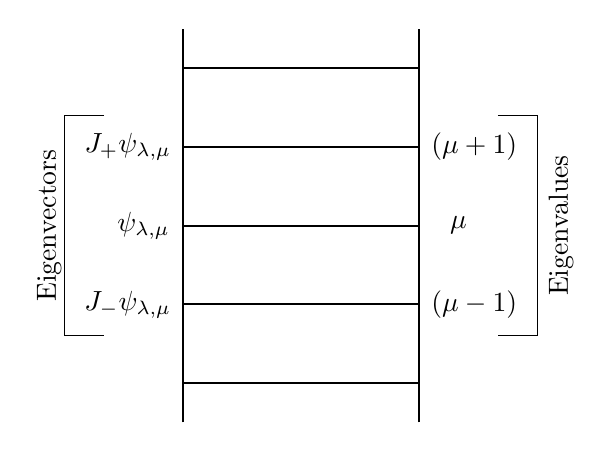
\begin{tikzpicture}
        \draw[thick] (0,0) -- (0,5); 
        \draw[thick] (3,0) -- (3,5);
        \draw[thick] (0,0.5) -- (3,0.5);
        \draw[thick] (0,1.5) -- (3,1.5);
        \draw[thick] (0,2.5) -- (3,2.5);
        \draw[thick] (0,3.5) -- (3,3.5);
        \draw[thick] (0,4.5) -- (3,4.5);
        %%%% 
        \node at (-0.5,2.5) {$\psi_{\lambda,\mu}$};
        \node at (-0.7,3.5) {$J_+\psi_{\lambda,\mu}$};
        \node at (-0.7,1.5) {$J_-\psi_{\lambda,\mu}$};
        \draw (-1, 3.9) -- (-1.5,3.9) -- (-1.5,1.1) -- (-1,1.1);
        \node[rotate = 90] at (-1.7,2.5) {Eigenvectors};
        \draw (4, 3.9) -- (4.5,3.9) -- (4.5,1.1) -- (4,1.1);
        \node[rotate = 90] at (4.8,2.5) {Eigenvalues};
        %%%%
        \node at (3.5,2.5) {$\mu$};
        \node at (3.7,3.5) {$(\mu+1)$};
        \node at (3.7,1.5) {$(\mu-1)$};
    \end{tikzpicture}
\end{center}
The next question would be is this a `proper' ladder; that is does it have a top and bottom rung or does it continue forever? The answer comes in the form of the next lemma. 
\er 

\bl 
There exists a $\psi_{\lambda,\overline{\mu}}$ such that $J_+\psi_{\lambda,\overline{\mu}} = 0$. Equally there exists a $\psi_{\lambda,\underline{\mu}}$ such that $J_-\psi_{\lambda,\underline{\mu}}=0$.  
\el 

\bq 
We know from \Cref{lem:CommonEigenvalueInequality} that $|\mu|(|\mu|+1) \leq \lambda$ holds for \emph{any} common eigenvector of $\Omega$ and $J_3$. We see from \Cref{lem:LadderEigenvalues} that $(J_{\pm})^n\psi_{\lambda,\mu}$ is such a common eigenvector, and so must obey $|\mu\pm n|(|\mu \pm n| +1)\leq \lambda$. However, $\lambda$ is unchanged by this repeated application of the ladder operators, and so, unless remedied,  this inequality will eventually be broken -- that is we need to somehow cap the available $n$ values. 

Consider first the raising operator. In this case $\mu+n$ gets bigger and bigger, and so we need to cap $n$ from above. In other words, we require there to be an $m\in\N$ such that for all $n > m$, $(J_+)^n\psi_{\lambda,\mu} = 0$. This fixes our problem as this corresponds to the zero vector and so, by definition, it cannot be a eigenvector, and the $\lambda$ inequality no longer need hold. We define 
\bse 
\psi_{\lambda,\overline{\mu}} := (J_+)^m\psi_{\lambda,\mu}.
\ese 

The idea is exactly the same is true for the lowering operator, however now $\mu-n$ is getting smaller and smaller, and so its modulus (after $n>\mu$ is reached) gets bigger and bigger. So again we need to cap $n$ from above. We require there to be a $\ell\in\N$ such that for all $n>\ell$, $(J_-)^n\psi_{\lambda,\mu}=0$. We define 
\bse 
\psi_{\lambda,\underline{\mu}} := (J_-)^{\ell} \psi_{\lambda,\mu}.
\ese 

Note we do not have any a priori relation between the values of $m$ and $\ell$. To use the ladder analogy, $m$ is the number of rungs above $\mu$-th rung and $\ell$ is the number of rungs below the $\mu$-th rung. For a given $\lambda$, the highest value of $\mu$ is denoted $\overline{\mu}(\lambda)$ and the lowest value $\underline{\mu}(\lambda)$. 
\eq 

\br 
Note the above tells us that $J_{\pm}\psi$ are not strictly eigenvalues, as it could be the zero vector. This is why we wrote `eigenvectors' in inverted commas in \Cref{lem:LadderEigenvalues}.
\er 

\bp 
The maximum and minimum values of $\mu$ satisfy 
\ben[label=(\roman*)]
\item $\lambda = \overline{\mu}(\lambda)\big(\overline{\mu}(\lambda)+1\big)$,
\item $\underline{\mu}(\lambda) = - \overline{\mu}(\lambda)$,
\item $\overline{\mu}(\lambda)\in\frac{\N_0}{2}$.
\een 
\ep 

\bq 
\ben[label=(\roman*)]
\item From the proof of \Cref{lem:CommonEigenvalueInequality}, and the fact that $J_+\psi_{\lambda,\overline{\mu}(\lambda)} = 0$, and so $\|J_+\psi_{\lambda,\overline{\mu}(\lambda)}\| = 0$, we have 
\bse
\lambda = \overline{\mu}(\lambda)\big(\overline{\mu}(\lambda)+1\big)
\ese
\item Repeating the above argument but with the fact that $\|J_-\psi_{\lambda,\underline{\mu}(\lambda)}\| = 0$, we have 
\bi{rCl}
\lambda & = & \underline{\mu}(\lambda)\big(\underline{\mu}(\lambda)-1\big) \\
& = & -\underline{\mu}(\lambda)\big(-\underline{\mu}(\lambda)+1\big),
\ei
and so $\underline{\mu}(\lambda) = -\overline{\mu}$.
\item From the previous, along with the fact that $\overline{\mu}(\lambda)-\underline{\mu}(\lambda) \in \N_0$ this result follows trivially.
\een 
\eq 

\br 
In order to be consistent with the literature we shall introduce the following relabelling 
\bse 
j := \overline{\mu}(\lambda), \qquad \qquad m := \mu.
\ese 
Note we have $j\in\frac{\N_0}{2}$.
\er 

\bt 
The \emph{common eigenvectors} of $\Omega$ and $J_3$ come as families $\psi_{j(j+1),m}$, where $m= -j,-j+1,...,j-1,j$. The eigenvalue $j(j+1)$ is associated to $\Omega$ and $m$ is associated to $J_3$.
\et 

One normally normalises these eigenvectors and defines 
\bse
\Phi_{j,m} := \frac{\psi_{j(j+1),m}}{\|\psi_{j(j+1),m}\|}.
\ese 
Then, from \Cref{lem:EigenvectorsOrthogonalDistinctEigenvalues} and the fact that the eigenvectors have distinct eigenvalues, we have 
\bse 
\braket{\Phi_{j,m}}{\Phi_{k,n}} = \delta_{jk}\delta_{mn}.
\ese 

\bc 
We have $m\in\frac{\Z}{2}$.
\ec 

\bq 
This comes from just allowing $j\in\frac{\N_0}{2}$ to be any element and then using $m=-j,...,j$. 
\eq 

\bp 
\label{prp:LadderCoefficients}
The the common eigenvectors $\Phi_{j,m}$ satisfy
\bi{rCl}
J_{\pm}\Phi_{j,m} = \sqrt{j(j+1) - m(m\pm1)}\Phi_{j,m\pm 1}.
\ei 
\ep 

\bq 
We shall show this for $J_+$, the method of $J_-$ follows analogously. Recall from \Cref{lem:CasimirLadder} that 
\bse  
J_-J_+ = \Omega - J_3(J_3+\id_{\cD}).
\ese
Now consider 
\bi{rCl}
\braket{J_+\Phi_{j,m}}{J_+\Phi_{j,m}} & = & \braket{\Phi_{j,m}}{J_-J_+\Phi_{j,m}} \\
& = & \braket{\Phi_{j,m}}{\Omega\Phi_{j,m}}  - \braket{\Phi_{j,m}}{J_3(J_3+\id_{\cD})\Phi_{j,m}} \\
& = & j(j+1) \braket{\Phi_{j,m}}{\Phi_{j,m}} - m(m+1)\braket{\Phi_{j,m}}{\Phi_{j,m}} \\
& = & j(j+1)-m(m+1).
\ei 
Combining this with \Cref{rem:LadderProportional} allows us to conclude the result. 
\eq 

\subsection{Pure Spin-$j$ Systems}

\bd 
A quantum mechanical system is called a \emph{pure spin-$j$} system if its Hilbert space is $(2j+1)$-dimensional that possesses an orthonormal eigenbasis $\{\Phi_{j,m}\}$ for the three operators $J_1,J_2,J_3$ defined on $\cH$.
\ed 

\bc 
The Hilbert space is isomorphic to $\C^{2j+1}$.
\ec 

\bc 
For a pure spin-$j$ system the spectrum of the operators is 
\bse
\sigma(J_i) = \{-j,-j+1,...,j-1,j\},
\ese 
for $i=1,2,3$.
\ec 

\be 
\hfill 

\begin{center}
    \begin{tabular}{c|c}
        $j$ & $\sigma(J_i)$, $i=1,2,3$ \\
         \hline $0$ & $0$ \\
         $1/2$ & $\{-1/2,1/2\}$ \\
         $1$ & $\{-1,0,1\}$
    \end{tabular}
\end{center}
\ee 

\br 
\label{rem:ElectronCompositeHilbert}
When you introduce spin to a particle, its Hilbert space becomes a product space. For example for an electron (spin-$1/2$) in $\R^3$ its Hilbert space is 
\bse
\cH_{e} = L^2(\R^3)\otimes \C^2.
\ese 
We shall return to this and expand on it in the next lecture.
\er 

\br 
You can also have non-pure spin systems. For the orbital angular momentum, you take a direct sum of the Hilbert spaces. That is if $\cH_j$ is the Hilbert space associated to the pure spin-$j$ system then the composite system's Hilbert space is 
\bse 
\cH_{comp} = \bigoplus_{j}\cH_j.
\ese 
We shall return to this in two lectures time.
\er 